\chapter{METHODOLOGY}
\section{Overview}
The project we are developing combines the power of voice recognition and computer vision to create a highly advanced and intuitive robotic system. Our robot is programmed in such a way that it recognizes the commands given by the operator, understands it and performs the specified operation which can be termed as human-robot interaction.

\section{Data Collection}
For the succession of our project, research and data collection played a major part. The methods used for collecting data required for our project included observations and secondary data analysis. By observing and experimenting the process we selected the suitable method. Similarly, all the documents and records available in the internet guided us throughout this project.
\section{Tools and Technologies}
\subsection{Hardware}
The project's hardware consists of a central control unit such as a Raspberry Pi. It also includes a robotic arm kit, an ultrasonic sensor for measuring distance, a camera module for computer vision tasks, motors, motor drivers, and peripheral like a microphone for voice interaction. These hardware components create the physical structure of the voice-controlled robot, enabling its mobility, sensing, and interaction with the surroundings.
\subsection{Software}
Python is the main programming language used for implementing the robot's functions in the project. OpenCV is utilized for computer vision tasks to help the robot understand its environment. TensorFlow is used to train the object detection model, which enables the robot to recognize and locate objects. Speech recognition libraries are incorporated to process voice commands for controlling the robot. Motor control libraries are also used to ensure precise movement of the robot, allowing it to perform tasks accurately. These software elements are essential for integrating voice control, computer vision, and robotic arm functions seamlessly within the robot system.
\section{System Block Diagram}
\begin{figure}[h]
    \centering
    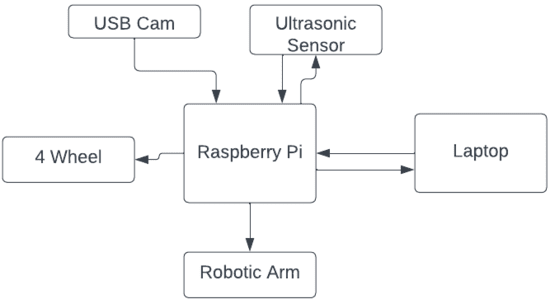
\includegraphics[width=1\linewidth]{systemBlockDiagram (1) (1).png}
    \caption{Voice Controlled Robot System Block Diagram}
    \label{fig:enter-label}
\end{figure}

\newpage
\section{System Flowchart}
\begin{figure}[h]
    \centering
    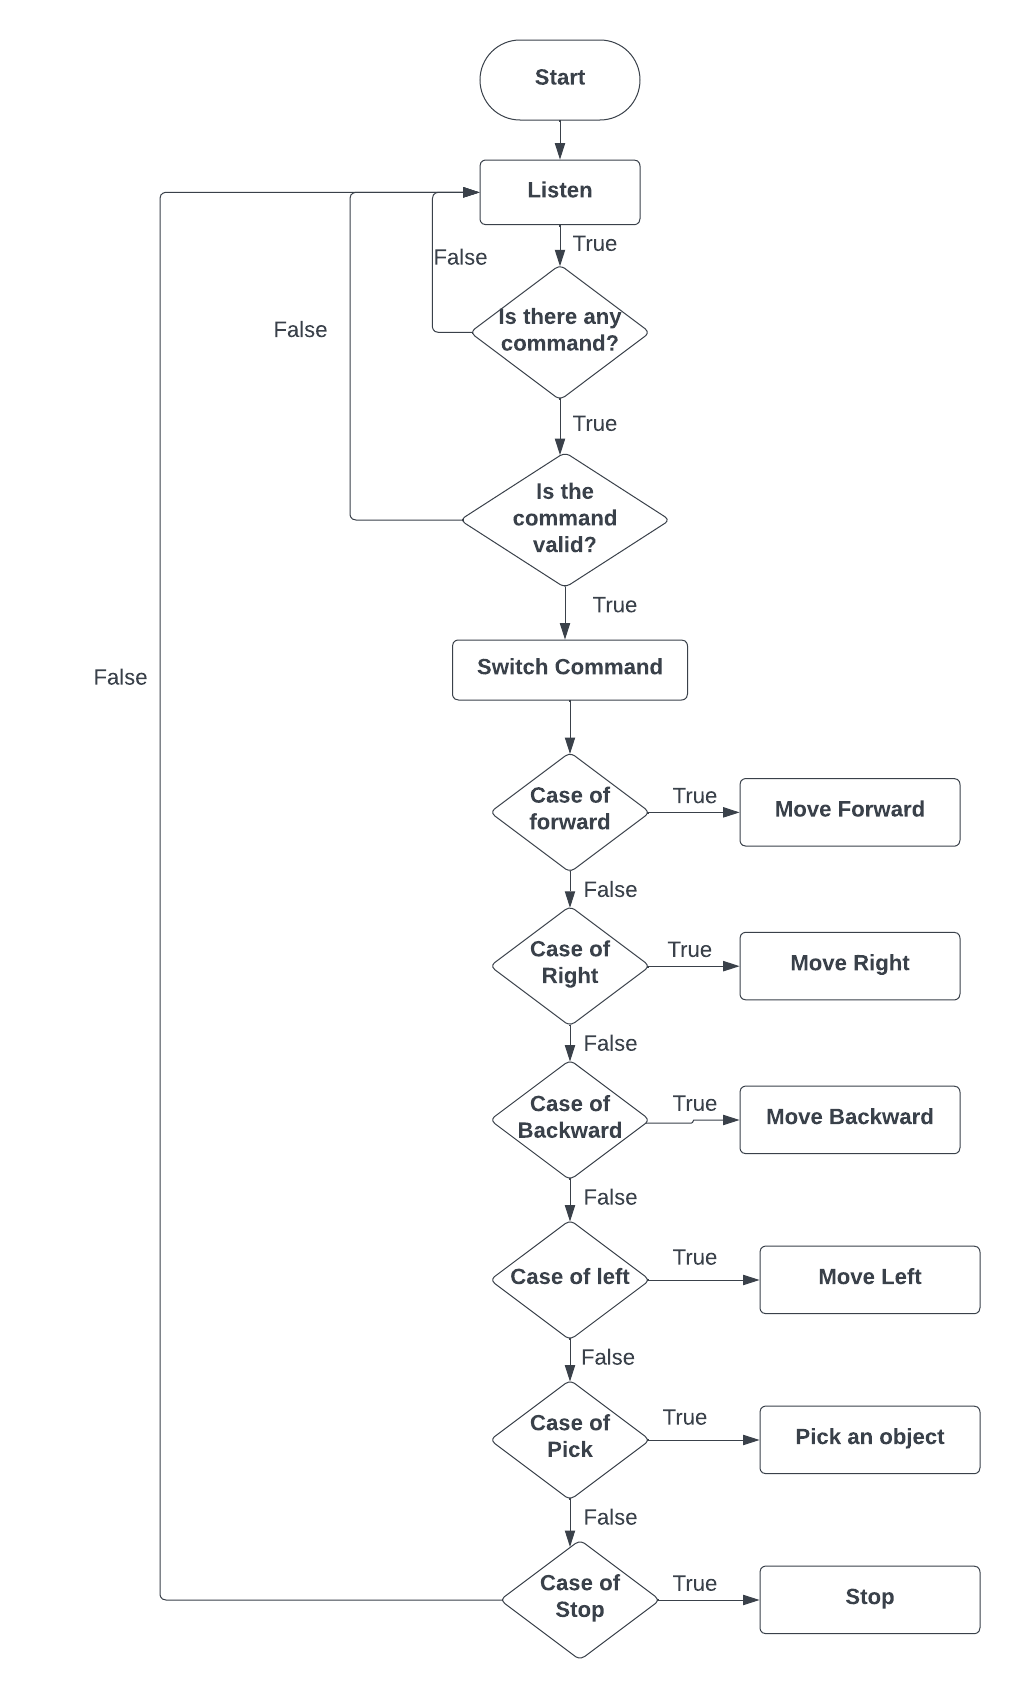
\includegraphics[width=0.7\linewidth]{systemFlowchart.png}
    \caption{System Flowchart}
    \label{fig:enter-label}
\end{figure}
\newpage
\section{Working Principle}
Our project is based on voice control and general AI robotics. The prime idea is to give 
commands to our robot and expect its performance accordingly. Our robot is 
programmed in such a way that it recognizes the commands given by the operator, 
understands it and performs the operation as specified by the operator. The operations 
can be vivid like: following the operator, moving in any direction as specified, picking 
various objects, etc. All-of these operations can be done with the help of computer 
vision, speech recognition, ML and a micro-controller like: Arduino. Although various 
other operations can be programmed, in our project we have programmed a few 
operations that will be seen in the robot's operations.
\section{Limitations}
\begin{itemize}
    \item \textbf{Speech Recognition Accuracy:} Voice recognition systems may not always 
accurately understand spoken commands, especially in noisy environments or with 
accents or speech variations. This can lead to misinterpretations and unintended 
actions by the robot.
    \item \textbf{Limited Vocabulary:}Training the speech recognition system to understand a vast 
vocabulary can be challenging. A limited set of recognized commands might 
restrict the robot's versatility and interactions with users. 
    \item \textbf{ Processing Time:}Real-time voice recognition and image processing can be 
computationally intensive, particularly on low-power microcontroller like those 
commonly used in robotics. This may lead to delays in response time and affect 
the robot's overall performance.
    \item \textbf{Recognition Complexity:}Object recognition algorithms may struggle with certain 
objects or in varying lighting conditions, leading to inaccurate or failed detection.
\end{itemize}
